\documentclass[10pt,twocolumn,a4paper]{article}
\usepackage[utf8]{inputenc}
\usepackage[T1]{fontenc}
\usepackage[brazil]{babel}
\usepackage[margin=2cm]{geometry}
\usepackage{amsmath,amssymb}
\usepackage{graphicx}
\usepackage{booktabs}
\usepackage{enumitem}
\usepackage{stfloats}
\usepackage[hidelinks]{hyperref}

\newcommand{\gitrepo}{https://github.com/GJakobi/ta03-transformacao-perspectiva}

\title{\textbf{Scanner de documentos com transformação perspectiva em OpenCV}}
\author{Gustavo Jakobi (GRR20221253) \and Bruno Crestani (GRR20221240)\\[2pt]
  \small Departamento de Informática -- Universidade Federal do Paraná (UFPR)\\
  \small Visão Computacional e Percepção -- Prof. Eduardo Todt\\
  \small Código: \url{\gitrepo}}
\date{}

\begin{document}
\maketitle

\begin{abstract}
Apresentamos um scanner de documentos baseado em homografia. A aplicação
encontra os 4 cantos de uma folha fotografada em ângulo, leva esses cantos a
um retângulo com \texttt{cv2.warpPerspective} e binariza o resultado. Em cinco
fotos sintéticas, o erro médio dos cantos ficou abaixo de 1{,}6~px. Numa foto
real, o documento saiu retificado e legível.
\end{abstract}

\section{Fundamentação}
Pontos de um plano e seus pontos na imagem estão relacionados por uma
homografia~\cite{hartley,szeliski,todt}. Em coordenadas homogêneas:
\begin{equation}
\begin{bmatrix}x'\\y'\\w'\end{bmatrix}=
\begin{bmatrix}a&b&c\\d&e&f\\g&h&1\end{bmatrix}
\begin{bmatrix}x\\y\\1\end{bmatrix},\quad
u=\frac{x'}{w'},\; v=\frac{y'}{w'}.
\end{equation}
A matriz tem 8 graus de liberdade. Cada par $(x,y)\rightarrow(u,v)$ gera duas
equações lineares, e 4 pares dão um sistema $8\times8$. A função
\texttt{getPerspectiveTransform} resolve este sistema~\cite{opencv}.

Como a folha é plana, uma única matriz $3\times3$ desfaz a perspectiva. Uma
transformação afim não basta: ela preserva o paralelismo e não leva um
trapézio a um retângulo (Figura~\ref{fig:afim}).

\begin{figure}[t]
\centering
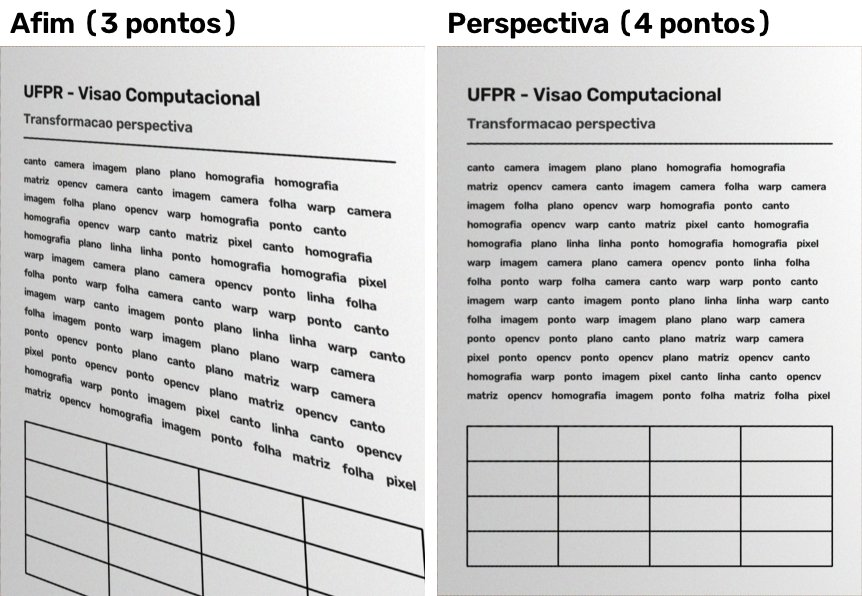
\includegraphics[width=\columnwidth]{figuras/afim_vs_perspectiva.jpg}
\caption{Mesma foto retificada com uma transformação afim (3 cantos) e com uma
homografia (4 cantos).}
\label{fig:afim}
\end{figure}

\section{Método}
\begin{enumerate}[leftmargin=*,itemsep=2pt]
\item \textbf{Detecção.} Reduzimos a imagem para 800~px de largura e aplicamos
um fechamento morfológico, que apaga o texto. Depois aplicamos Canny e
escolhemos o maior contorno que \texttt{approxPolyDP} reduz a 4 vértices
(Figura~\ref{fig:pipeline}).
\item \textbf{Alternativa por Hough.} Se nenhum contorno fecha, aplicamos
\texttt{HoughLinesP} e guardamos os segmentos longos. Os segmentos mais
externos em cada direção são os 4 lados, e os cantos são as interseções.
\item \textbf{Refinamento.} Na resolução cheia, ajustamos uma reta a cada lado
com \texttt{fitLine}. Cada canto é a interseção de dois lados vizinhos:
$\mathbf{x}=\mathbf{l}_1\times\mathbf{l}_2$.
\item \textbf{Warp.} Calculamos $\mathbf{H}$ e aplicamos
\texttt{warpPerspective}. O tamanho de saída é o maior comprimento de cada
par de lados opostos.
\item \textbf{Efeito de scanner.} Dividimos a imagem pelo fundo estimado, para
remover sombras, e aplicamos \texttt{adaptiveThreshold}.
\end{enumerate}
Se a detecção falhar, a opção \texttt{-{}-manual} permite clicar nos 4 cantos.

\begin{figure*}[t]
\centering
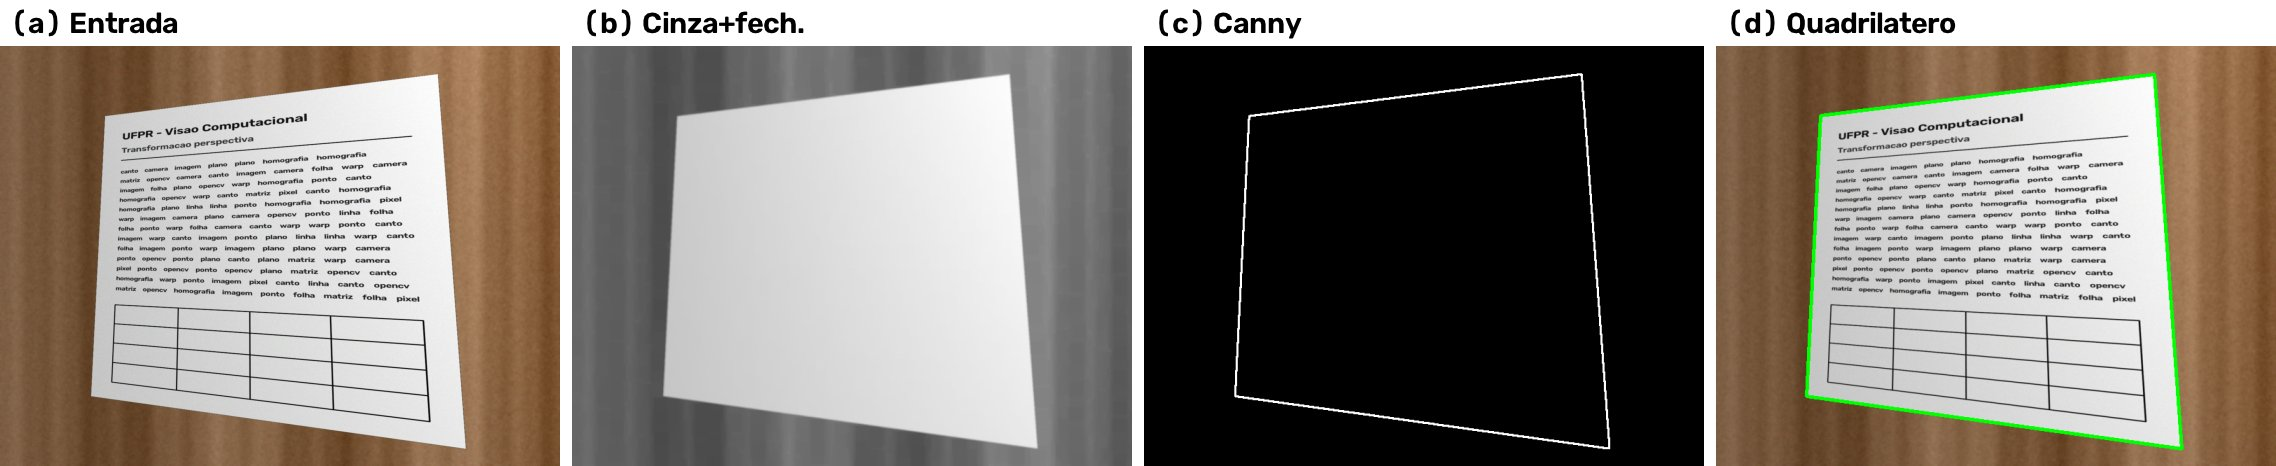
\includegraphics[width=\textwidth]{figuras/pipeline.jpg}
\caption{Detecção: (a) entrada; (b) cinza após o fechamento; (c) Canny;
(d) quadrilátero encontrado.}
\label{fig:pipeline}
\end{figure*}

\section{Experimentos e resultados}
Geramos cinco fotos sintéticas com cantos conhecidos. Um documento é projetado
sobre um fundo de madeira com iluminação desigual, ruído e compressão JPEG.
Medimos o erro médio dos cantos e a correlação cruzada normalizada (NCC) entre
o documento retificado e o original. NCC~$=1$ indica imagens iguais.

\begin{table*}[t]
\centering
\caption{Resultados nas fotos sintéticas. ``Cantos reais'' é a NCC com os
cantos verdadeiros (limite superior).}
\label{tab:res}
\begin{tabular}{lcccccc}
\toprule
 & \multicolumn{2}{c}{Erro dos cantos (px)} & \multicolumn{3}{c}{NCC} & \\
\cmidrule(lr){2-3}\cmidrule(lr){4-6}
Caso & sem refino & com refino & sem refino & com refino & cantos reais & $\max|H_{\text{nosso}}-H_{\text{cv}}|$\\
\midrule
\csname @@input\endcsname tabela.tex
\bottomrule
\end{tabular}
\end{table*}


A detecção encontrou a folha nos cinco casos (Tabela~\ref{tab:res}). Sem refinamento, o erro ficou em cerca de 2~px; no
caso de perspectiva forte, um canto errou 68~px. O refinamento reduziu o erro
para menos de 0{,}5~px em quatro casos e para 1{,}6~px no caso mais difícil.
A NCC ficou perto do limite dado pelos cantos reais. No caso de perspectiva
forte, a borda distante ocupa poucos pixels, e a homografia amplia qualquer
erro nessa região. Nosso sistema $8\times8$ e o OpenCV deram a mesma matriz,
com diferença abaixo de $10^{-12}$.

\begin{figure*}[b]
\centering
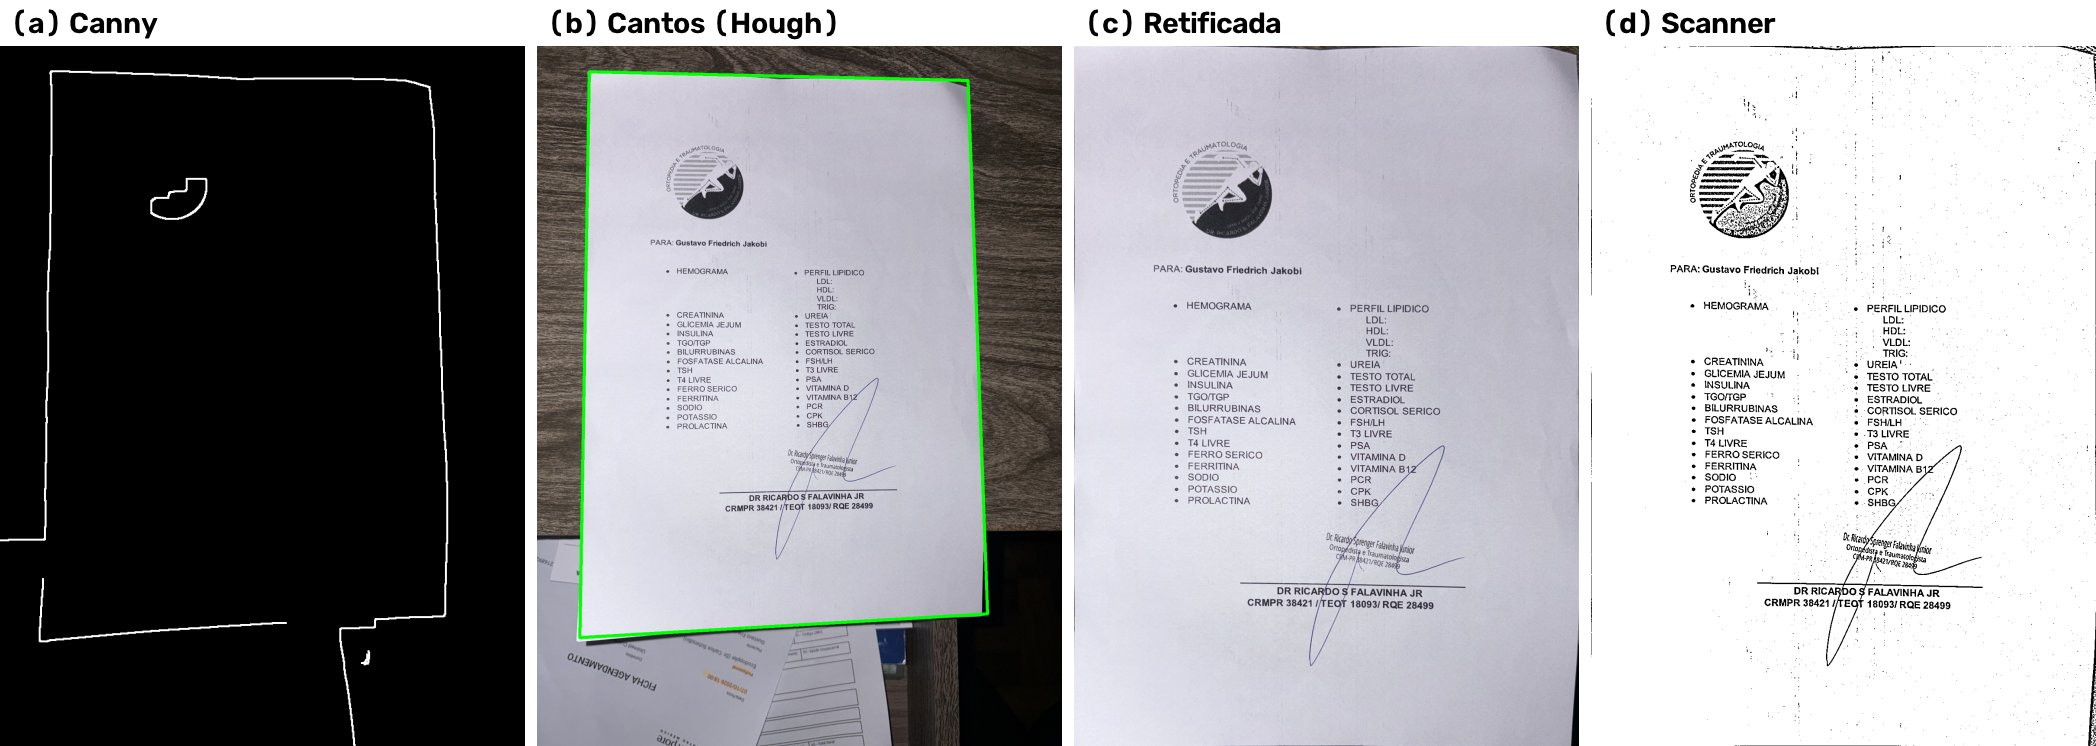
\includegraphics[width=\textwidth]{figuras/foto_real.jpg}
\caption{Foto real: (a) Canny, com falhas na borda onde a folha encosta em
outro papel; (b) cantos por Hough; (c) retificada; (d) efeito de scanner.}
\label{fig:real}
\end{figure*}

\paragraph{Foto real.} Testamos uma foto de celular de uma folha A4 sobre
outros papéis brancos (Figura~\ref{fig:real}). O contorno não fechou, mas a
etapa de Hough encontrou os 4 lados, e o documento saiu legível. A folha
estava um pouco curvada, e a homografia só corrige superfícies planas.

\section{Conclusão}
Uma homografia calculada com 4 pontos remove a perspectiva de um objeto plano.
A parte difícil é encontrar os cantos com precisão: o ajuste de retas reduziu
o erro para menos de 2~px em todos os casos. A detecção falha quando a folha
não contrasta com o fundo; nesse caso, o modo manual resolve.

\begin{thebibliography}{9}
\bibitem{hartley} R. Hartley e A. Zisserman. \emph{Multiple View Geometry in
Computer Vision}. 2.~ed. Cambridge University Press, 2004.
\bibitem{szeliski} R. Szeliski. \emph{Computer Vision: Algorithms and
Applications}. 2.~ed. Springer, 2022.
\bibitem{opencv} OpenCV. \emph{Geometric Transformations of Images}.
\url{https://docs.opencv.org/4.x/da/d6e/tutorial_py_geometric_transformations.html}.
\bibitem{todt} E. Todt. \emph{Transformations and warping}. Notas de aula,
Visão Computacional e Percepção, UFPR, 2026.
\end{thebibliography}

\end{document}
